\documentclass[tikz,border=10pt]{standalone}

\begin{document}


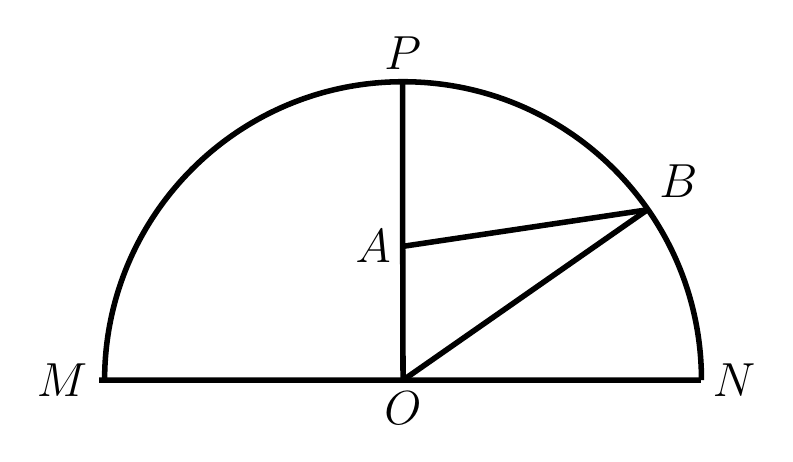
\begin{tikzpicture}[line join=round, line width=2.0pt,
  every node/.style={font=\fontsize{19}{23}\selectfont}]
\coordinate (A) at (0.000,-0.179);
\coordinate (B) at (3.106,0.285);
\coordinate (M) at (-3.855,-1.879);
\coordinate (N) at (3.788,-1.879);
\coordinate (O) at (0.004,-1.878);
\coordinate (P) at (0.000,1.914);








  
  \draw (O) ++(180.000:3.790) arc[start angle=180.000, end angle=0.000, radius=3.790];

  
  \draw (M) -- (O) -- (N);

  
  \draw (O) -- (A) -- (P);

  
  \draw (O) -- (B);
  \draw (A) -- (B);

  
  \node[left] at (M) {$M$};
  \node[right] at (N) {$N$};
  \node[above] at (P) {$P$};
  \node[below] at (O) {$O$};
  \node[left] at (A) {$A$};
  \node[above right] at (B) {$B$};
\end{tikzpicture}
\end{document}